\chapter{Date and Time}\label{introduction-to-python---lesson-3}

\begin{Exercise}[label={dateex}]
Write code that:

\begin{itemize}
\item print the day of the week of your birthday
\item print the weekday of your birthdays for the next 120 years
\end{itemize}
\end{Exercise}

\begin{Answer}
\begin{codebox}[size=fbox, boxrule=1pt, colback=cellbackground, colframe=cellborder]
\begin{Verbatim}[commandchars=\\\{\}]
\PY{k+kn}{import} \PY{n+nn}{datetime}

\PY{n}{birthday} \PY{o}{=} \PY{n}{datetime}\PY{o}{.}\PY{n}{date}\PY{p}{(}\PY{l+m+mi}{1974}\PY{p}{,} \PY{l+m+mi}{10}\PY{p}{,} \PY{l+m+mi}{20}\PY{p}{)}
\PY{n+nb}{print} \PY{p}{(}\PY{n}{birthday}\PY{o}{.}\PY{n}{weekday}\PY{p}{(}\PY{p}{)}\PY{p}{)} \PY{c+c1}{\PYZsh{} remember it starts form 0}

6
\end{Verbatim}
\end{codebox}

\begin{codebox}[size=fbox, boxrule=1pt, colback=cellbackground, colframe=cellborder]
\begin{Verbatim}[commandchars=\\\{\}]
\PY{k+kn}{from} \PY{n+nn}{dateutil}\PY{n+nn}{.}\PY{n+nn}{relativedelta} \PY{k}{import} \PY{n}{relativedelta}

\PY{k}{for} \PY{n}{i} \PY{o+ow}{in} \PY{n+nb}{range}\PY{p}{(}\PY{l+m+mi}{120}\PY{p}{)}\PY{p}{:}
    \PY{n+nb}{print} \PY{p}{(}\PY{p}{(}\PY{n}{birthday} \PY{o}{+} \PY{n}{relativedelta}\PY{p}{(}\PY{n}{years}\PY{o}{=}\PY{n}{i}\PY{p}{)}\PY{p}{)}\PY{o}{.}\PY{n}{weekday}\PY{p}{(}\PY{p}{)}\PY{p}{)}

6
0
2
3
4
5
0
1
2
3
4
...
\end{Verbatim}
\end{codebox}
\end{Answer}

\begin{Exercise}
  Write code to determine whether a given year is a leap year and test it with 1800, 1987 and 2020.
  \textbf{Hint:} a leap year is divisible by 4, by 100 and by 400.
\end{Exercise}

\begin{Answer}
\begin{codebox}[size=fbox, boxrule=1pt, colback=cellbackground, colframe=cellborder]
\begin{Verbatim}[commandchars=\\\{\}]
\PY{n}{years} \PY{o}{=} \PY{p}{[}\PY{l+m+mi}{1800}\PY{p}{,} \PY{l+m+mi}{1987}\PY{p}{,} \PY{l+m+mi}{2020}\PY{p}{]}

\PY{k}{for} \PY{n}{y} \PY{o+ow}{in} \PY{n}{years}\PY{p}{:}
    \PY{k}{if} \PY{n}{y} \PY{o}{\PYZpc{}} \PY{l+m+mi}{400} \PY{o}{==} \PY{l+m+mi}{0}\PY{p}{:}
        \PY{n+nb}{print} \PY{p}{(}\PY{l+s+s2}{\PYZdq{}}\PY{l+s+si}{\PYZob{}\PYZcb{}}\PY{l+s+s2}{ is a leap year }\PY{l+s+s2}{\PYZdq{}}\PY{o}{.}\PY{n}{format}\PY{p}{(}\PY{n}{y}\PY{p}{)}\PY{p}{)}
    \PY{k}{elif} \PY{n}{y} \PY{o}{\PYZpc{}} \PY{l+m+mi}{100} \PY{o}{==} \PY{l+m+mi}{0}\PY{p}{:}
        \PY{n+nb}{print} \PY{p}{(}\PY{l+s+s2}{\PYZdq{}}\PY{l+s+si}{\PYZob{}\PYZcb{}}\PY{l+s+s2}{ is NOT a leap year }\PY{l+s+s2}{\PYZdq{}}\PY{o}{.}\PY{n}{format}\PY{p}{(}\PY{n}{y}\PY{p}{)}\PY{p}{)}
    \PY{k}{elif} \PY{n}{y} \PY{o}{\PYZpc{}} \PY{l+m+mi}{4} \PY{o}{==} \PY{l+m+mi}{0}\PY{p}{:}
        \PY{n+nb}{print} \PY{p}{(}\PY{l+s+s2}{\PYZdq{}}\PY{l+s+si}{\PYZob{}\PYZcb{}}\PY{l+s+s2}{ is a leap year }\PY{l+s+s2}{\PYZdq{}}\PY{o}{.}\PY{n}{format}\PY{p}{(}\PY{n}{y}\PY{p}{)}\PY{p}{)}
    \PY{k}{else}\PY{p}{:}
        \PY{n+nb}{print} \PY{p}{(}\PY{l+s+s2}{\PYZdq{}}\PY{l+s+si}{\PYZob{}\PYZcb{}}\PY{l+s+s2}{ is NOT a leap year }\PY{l+s+s2}{\PYZdq{}}\PY{o}{.}\PY{n}{format}\PY{p}{(}\PY{n}{y}\PY{p}{)}\PY{p}{)}

1800 is NOT a leap year
1987 is NOT a leap year
2020 is a leap year        
\end{Verbatim}
\end{codebox}  
\end{Answer}

\begin{Exercise}
Write code to print next five days starting from today.
\end{Exercise}

\begin{Answer}
\begin{codebox}[size=fbox, boxrule=1pt, colback=cellbackground, colframe=cellborder]
\begin{Verbatim}[commandchars=\\\{\}]
\PY{n}{d} \PY{o}{=} \PY{n}{datetime}\PY{o}{.}\PY{n}{date}\PY{o}{.}\PY{n}{today}\PY{p}{(}\PY{p}{)}
\PY{k}{for} \PY{n}{i} \PY{o+ow}{in} \PY{n+nb}{range}\PY{p}{(}\PY{l+m+mi}{1}\PY{p}{,} \PY{l+m+mi}{6}\PY{p}{)}\PY{p}{:}
    \PY{n+nb}{print} \PY{p}{(}\PY{n}{d} \PY{o}{+} \PY{n}{relativedelta}\PY{p}{(}\PY{n}{days}\PY{o}{=}\PY{n}{i}\PY{p}{)}\PY{p}{)}

2020-08-04
2020-08-05
2020-08-06
2020-08-07
2020-08-08
\end{Verbatim}
\end{codebox}
\end{Answer}

\begin{Exercise}
Build again dates as in Exercise~\ref{dateex} (i.e. the weekday of your birthdays for the next 120 years) and count how many of your birthdays is a Monday, Tuesday, \ldots{} , Sunday until 120 years of age. Print out the result using a dictionary. (expected output something like: \texttt{\{6:\ 10,\ 0:\ 10,\ 2:\ 9,\ 3:\ 10,\ 4:\ 10,\ 5:\ 10,\ 1:\ 9\}})
\end{Exercise}

\begin{Answer}
\begin{codebox}[size=fbox, boxrule=1pt, colback=cellbackground, colframe=cellborder]
\begin{Verbatim}[commandchars=\\\{\}]
\PY{k+kn}{import} \PY{n+nn}{datetime}
\PY{k+kn}{from} \PY{n+nn}{dateutil}\PY{n+nn}{.}\PY{n+nn}{relativedelta} \PY{k}{import} \PY{n}{relativedelta}
\PY{n}{birthday} \PY{o}{=} \PY{n}{datetime}\PY{o}{.}\PY{n}{date}\PY{p}{(}\PY{l+m+mi}{1974}\PY{p}{,} \PY{l+m+mi}{10}\PY{p}{,} \PY{l+m+mi}{20}\PY{p}{)}

\PY{n}{d} \PY{o}{=} \PY{p}{\PYZob{}}\PY{p}{\PYZcb{}}
\PY{k}{for} \PY{n}{i} \PY{o+ow}{in} \PY{n+nb}{range}\PY{p}{(}\PY{l+m+mi}{120}\PY{p}{)}\PY{p}{:}
    \PY{n}{wd} \PY{o}{=} \PY{p}{(}\PY{p}{(}\PY{n}{birthday} \PY{o}{+} \PY{n}{relativedelta}\PY{p}{(}\PY{n}{years}\PY{o}{=}\PY{n}{i}\PY{p}{)}\PY{p}{)}\PY{o}{.}\PY{n}{weekday}\PY{p}{(}\PY{p}{)}\PY{p}{)}
    \PY{k}{if} \PY{n}{wd} \PY{o+ow}{in} \PY{n}{d}\PY{o}{.}\PY{n}{keys}\PY{p}{(}\PY{p}{)}\PY{p}{:}
        \PY{n}{d}\PY{p}{[}\PY{n}{wd}\PY{p}{]} \PY{o}{=} \PY{n}{d}\PY{p}{[}\PY{n}{wd}\PY{p}{]} \PY{o}{+} \PY{l+m+mi}{1}
    \PY{k}{else}\PY{p}{:}
        \PY{n}{d}\PY{p}{[}\PY{n}{wd}\PY{p}{]} \PY{o}{=} \PY{l+m+mi}{1}
        
\PY{n+nb}{print} \PY{p}{(}\PY{n}{d}\PY{p}{)}

\{6: 17, 0: 18, 2: 17, 3: 17, 4: 17, 5: 17, 1: 17\}
\end{Verbatim}
\end{codebox}
\end{Answer}

\begin{Exercise}[label={ex:date_series}, title={(Date Generator)}]
In the next lessons we will create many contracts (e.g. swaps) which take in input lists of dates like for example the payment dates. Since it would be very boring to write long list of dates for each of these contracts, the goal of this exercise is to write code which given a start date and a number of months, returns a list of dates of \textbf{annual} frequency from the start date to the ending of the period after the specified number of months.

For example
\begin{itemize}
\item 2019-11-10 start date 12 months \(\rightarrow\) 2019-11-10, 2020-11-10
\item 2019-11-10 start date 24 months \(\rightarrow\) 2019-11-10, 2020-11-10, 2021-11-10
\end{itemize}

Note that if the number of months is not a multiple of 12, the last period should simply be shorter than 12 months. For example:

\begin{itemize}
\item 2019-11-10 start date 9 months \(\rightarrow\) 2019-11-10, 2020-08-10
\item 2019-11-10 start date 15 months \(\rightarrow\) 2019-11-10, 2020-11-10, 2021-02-10
\end{itemize}

Once you have done save this code in a file called \texttt{finmarkets.py}, this will become our financial library and will be extended and used later on.
%\begin{figure}
%  %\centering
%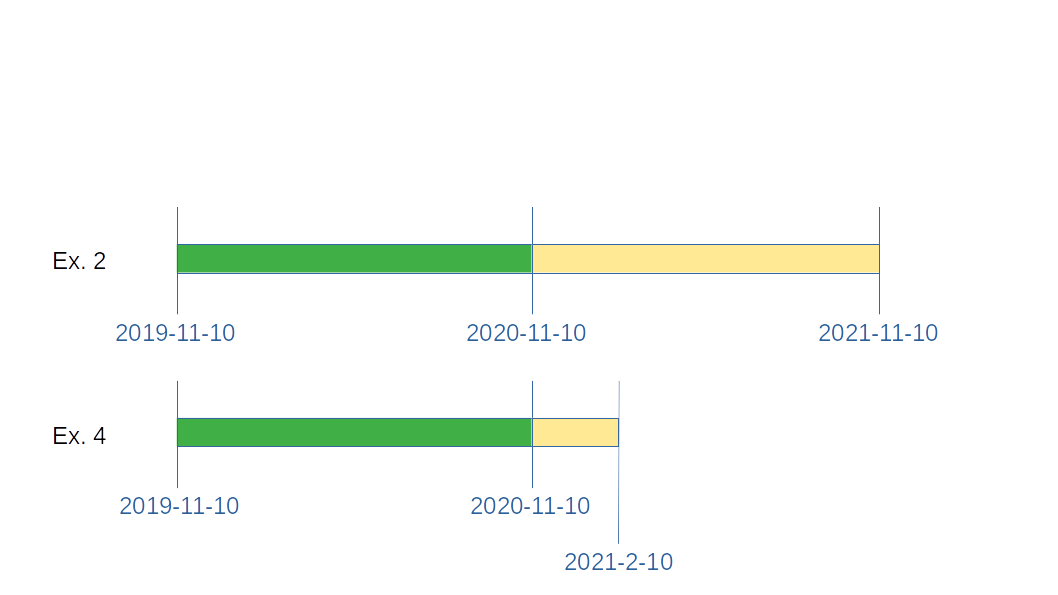
\includegraphics[width=0.8\linewidth]{time_flow.png}
%\end{figure}

%Here's some skeleton code to help you get started:
%
%\begin{Shaded}
%\begin{Highlighting}[]
%\ImportTok{from}\NormalTok{ dateutil }\ImportTok{import}\NormalTok{ relativedelta}
%
%\KeywordTok{def}\NormalTok{ generate_swap_dates(start_date, n_months):}
%\NormalTok{    dates }\OperatorTok{=}\NormalTok{ []}
%    \CommentTok{# your code here which adds all the relevant dates to the dates list}
%    \ControlFlowTok{return}\NormalTok{ dates}
%\end{Highlighting}
%\end{Shaded}
%
%\begin{Shaded}
%\begin{Highlighting}[]
%\CommentTok{# some tests to check if the function is working correctly}
%\ImportTok{from}\NormalTok{ datetime }\ImportTok{import}\NormalTok{ date}
%
%\ControlFlowTok{assert}\NormalTok{ generate_swap_dates(date(}\DecValTok{2019}\NormalTok{, }\DecValTok{11}\NormalTok{, }\DecValTok{10}\NormalTok{), }\DecValTok{12}\NormalTok{) }\OperatorTok{==}\NormalTok{ [date(}\DecValTok{2019}\NormalTok{, }\DecValTok{11}\NormalTok{, }\DecValTok{10}\NormalTok{), }
%\NormalTok{                                                       date(}\DecValTok{2020}\NormalTok{, }\DecValTok{11}\NormalTok{, }\DecValTok{10}\NormalTok{)]}
%\ControlFlowTok{assert}\NormalTok{ generate_swap_dates(date(}\DecValTok{2019}\NormalTok{, }\DecValTok{11}\NormalTok{, }\DecValTok{10}\NormalTok{), }\DecValTok{24}\NormalTok{) }\OperatorTok{==}\NormalTok{ [date(}\DecValTok{2019}\NormalTok{, }\DecValTok{11}\NormalTok{, }\DecValTok{10}\NormalTok{), }
%\NormalTok{                                                       date(}\DecValTok{2020}\NormalTok{, }\DecValTok{11}\NormalTok{, }\DecValTok{10}\NormalTok{), }
%\NormalTok{                                                       date(}\DecValTok{2021}\NormalTok{, }\DecValTok{11}\NormalTok{, }\DecValTok{10}\NormalTok{)]}
%
%\ControlFlowTok{assert}\NormalTok{ generate_swap_dates(date(}\DecValTok{2019}\NormalTok{, }\DecValTok{11}\NormalTok{, }\DecValTok{10}\NormalTok{), }\DecValTok{9}\NormalTok{) }\OperatorTok{==}\NormalTok{ [date(}\DecValTok{2019}\NormalTok{, }\DecValTok{11}\NormalTok{, }\DecValTok{10}\NormalTok{), }
%\NormalTok{                                                      date(}\DecValTok{2020}\NormalTok{, }\DecValTok{8}\NormalTok{, }\DecValTok{10}\NormalTok{)]}
%\ControlFlowTok{assert}\NormalTok{ generate_swap_dates(date(}\DecValTok{2019}\NormalTok{, }\DecValTok{11}\NormalTok{, }\DecValTok{10}\NormalTok{), }\DecValTok{15}\NormalTok{) }\OperatorTok{==}\NormalTok{ [date(}\DecValTok{2019}\NormalTok{, }\DecValTok{11}\NormalTok{, }\DecValTok{10}\NormalTok{), }
%\NormalTok{                                                       date(}\DecValTok{2020}\NormalTok{, }\DecValTok{11}\NormalTok{, }\DecValTok{10}\NormalTok{), }
%\NormalTok{                                                       date(}\DecValTok{2021}\NormalTok{, }\DecValTok{2}\NormalTok{, }\DecValTok{10}\NormalTok{)]}
%\end{Highlighting}
%\end{Shaded}
\end{Exercise}
\vfill
\begin{Answer}
\begin{codebox}[size=fbox, boxrule=1pt, colback=cellbackground, colframe=cellborder]
\begin{Verbatim}[commandchars=\\\{\}]
\PY{k+kn}{from} \PY{n+nn}{finmarkets} \PY{k}{import} \PY{n}{generate\PYZus{}swap\PYZus{}dates}
\PY{k+kn}{from} \PY{n+nn}{datetime} \PY{k}{import} \PY{n}{date}
\PY{k+kn}{from} \PY{n+nn}{dateutil}\PY{n+nn}{.}\PY{n+nn}{relativedelta} \PY{k}{import} \PY{n}{relativedelta}

\PY{n}{start_dates} \PY{o}{=} \PY{n}{date}\PY{p}{(}\PY{l+m+mi}{2019}\PY{p}{,} \PY{l+m+mi}{11}\PY{p}{,} \PY{l+m+mi}{10}\PY{p}{)}
\PY{n}{n\_months} \PY{o}{=} \PY{l+m+mi}{15}
\PY{n}{dates} \PY{o}{=} \PY{p}{[}\PY{p}{]}
\PY{k}{for} \PY{n}{i} \PY{o+ow}{in} \PY{n+nb}{range}\PY{p}{(}\PY{l+m+mi}{0}\PY{p}{,} \PY{n}{n\PYZus{}months}\PY{p}{,} \PY{l+m+mi}{12}\PY{p}{)}\PY{p}{:}
    \PY{n}{dates}\PY{o}{.}\PY{n}{append}\PY{p}{(}\PY{n}{start\PYZus{}date} \PY{o}{+} \PY{n}{relativedelta}\PY{p}{(}\PY{n}{months}\PY{o}{=}\PY{n}{i}\PY{p}{)}\PY{p}{)}
\PY{n}{dates}\PY{o}{.}\PY{n}{append}\PY{p}{(}\PY{n}{start\PYZus{}date} \PY{o}{+} \PY{n}{relativedelta}\PY{p}{(}\PY{n}{months}\PY{o}{=}\PY{n}{n\PYZus{}months}\PY{p}{)}\PY{p}{)}

\PY{k}{print}\PY{p}{(}\PY{n}{dates}\PY{p}{)}

\PY{p}{[}\PY{n}{date}\PY{p}{(}\PY{l+m+mi}{2019}\PY{p}{,} \PY{l+m+mi}{11}\PY{p}{,} \PY{l+m+mi}{10}\PY{p}{)}\PY{p}{,} 
 \PY{n}{date}\PY{p}{(}\PY{l+m+mi}{2020}\PY{p}{,} \PY{l+m+mi}{11}\PY{p}{,} \PY{l+m+mi}{10}\PY{p}{)}\PY{p}{,} 
 \PY{n}{date}\PY{p}{(}\PY{l+m+mi}{2021}\PY{p}{,} \PY{l+m+mi}{2}\PY{p}{,} \PY{l+m+mi}{10}\PY{p}{)}\PY{p}{]}
\end{Verbatim}
\end{codebox}
\end{Answer}

%\begin{Answer}
%\begin{Verbatim}[commandchars=\\\{\}]
%\PY{k+kn}{from} \PY{n+nn}{finmarkets} \PY{k}{import} \PY{n}{generate\PYZus{}swap\PYZus{}dates}
%\PY{k+kn}{from} \PY{n+nn}{datetime} \PY{k}{import} \PY{n}{date}
%\PY{k+kn}{from} \PY{n+nn}{dateutil}\PY{n+nn}{.}\PY{n+nn}{relativedelta} \PY{k}{import} \PY{n}{relativedelta}
%
%\PY{k}{def} \PY{n+nf}{generate\PYZus{}swap\PYZus{}dates}\PY{p}{(}\PY{n}{start\PYZus{}date}\PY{p}{,} \PY{n}{n\PYZus{}months}\PY{p}{)}\PY{p}{:}
%    \PY{n}{dates} \PY{o}{=} \PY{p}{[}\PY{p}{]}
%    \PY{k}{for} \PY{n}{i} \PY{o+ow}{in} \PY{n+nb}{range}\PY{p}{(}\PY{l+m+mi}{0}\PY{p}{,} \PY{n}{n\PYZus{}months}\PY{p}{,} \PY{l+m+mi}{12}\PY{p}{)}\PY{p}{:}
%        \PY{n}{dates}\PY{o}{.}\PY{n}{append}\PY{p}{(}\PY{n}{start\PYZus{}date} \PY{o}{+} \PY{n}{relativedelta}\PY{p}{(}\PY{n}{months}\PY{o}{=}\PY{n}{i}\PY{p}{)}\PY{p}{)}
%    \PY{n}{dates}\PY{o}{.}\PY{n}{append}\PY{p}{(}\PY{n}{start\PYZus{}date} \PY{o}{+} \PY{n}{relativedelta}\PY{p}{(}\PY{n}{months}\PY{o}{=}\PY{n}{n\PYZus{}months}\PY{p}{)}\PY{p}{)}
%    
%    \PY{k}{return} \PY{n}{dates}
%
%
%\PY{k}{assert} \PY{n}{generate\PYZus{}swap\PYZus{}dates}\PY{p}{(}\PY{n}{date}\PY{p}{(}\PY{l+m+mi}{2019}\PY{p}{,} \PY{l+m+mi}{11}\PY{p}{,} \PY{l+m+mi}{10}\PY{p}{)}\PY{p}{,} \PY{l+m+mi}{12}\PY{p}{)} \PY{o}{==} \PY{p}{[}\PY{n}{date}\PY{p}{(}\PY{l+m+mi}{2019}\PY{p}{,} \PY{l+m+mi}{11}\PY{p}{,} \PY{l+m+mi}{10}\PY{p}{)}\PY{p}{,} 
%                                                       \PY{n}{date}\PY{p}{(}\PY{l+m+mi}{2020}\PY{p}{,} \PY{l+m+mi}{11}\PY{p}{,} \PY{l+m+mi}{10}\PY{p}{)}\PY{p}{]}
%\PY{k}{assert} \PY{n}{generate\PYZus{}swap\PYZus{}dates}\PY{p}{(}\PY{n}{date}\PY{p}{(}\PY{l+m+mi}{2019}\PY{p}{,} \PY{l+m+mi}{11}\PY{p}{,} \PY{l+m+mi}{10}\PY{p}{)}\PY{p}{,} \PY{l+m+mi}{24}\PY{p}{)} \PY{o}{==} \PY{p}{[}\PY{n}{date}\PY{p}{(}\PY{l+m+mi}{2019}\PY{p}{,} \PY{l+m+mi}{11}\PY{p}{,} \PY{l+m+mi}{10}\PY{p}{)}\PY{p}{,} 
%                                                       \PY{n}{date}\PY{p}{(}\PY{l+m+mi}{2020}\PY{p}{,} \PY{l+m+mi}{11}\PY{p}{,} \PY{l+m+mi}{10}\PY{p}{)}\PY{p}{,} 
%                                                       \PY{n}{date}\PY{p}{(}\PY{l+m+mi}{2021}\PY{p}{,} \PY{l+m+mi}{11}\PY{p}{,} \PY{l+m+mi}{10}\PY{p}{)}\PY{p}{]}
%
%\PY{k}{assert} \PY{n}{generate\PYZus{}swap\PYZus{}dates}\PY{p}{(}\PY{n}{date}\PY{p}{(}\PY{l+m+mi}{2019}\PY{p}{,} \PY{l+m+mi}{11}\PY{p}{,} \PY{l+m+mi}{10}\PY{p}{)}\PY{p}{,} \PY{l+m+mi}{9}\PY{p}{)} \PY{o}{==} \PY{p}{[}\PY{n}{date}\PY{p}{(}\PY{l+m+mi}{2019}\PY{p}{,} \PY{l+m+mi}{11}\PY{p}{,} \PY{l+m+mi}{10}\PY{p}{)}\PY{p}{,} 
%                                                      \PY{n}{date}\PY{p}{(}\PY{l+m+mi}{2020}\PY{p}{,} \PY{l+m+mi}{8}\PY{p}{,} \PY{l+m+mi}{10}\PY{p}{)}\PY{p}{]}
%\PY{k}{assert} \PY{n}{generate\PYZus{}swap\PYZus{}dates}\PY{p}{(}\PY{n}{date}\PY{p}{(}\PY{l+m+mi}{2019}\PY{p}{,} \PY{l+m+mi}{11}\PY{p}{,} \PY{l+m+mi}{10}\PY{p}{)}\PY{p}{,} \PY{l+m+mi}{15}\PY{p}{)} \PY{o}{==} \PY{p}{[}\PY{n}{date}\PY{p}{(}\PY{l+m+mi}{2019}\PY{p}{,} \PY{l+m+mi}{11}\PY{p}{,} \PY{l+m+mi}{10}\PY{p}{)}\PY{p}{,} 
%                                                               \PY{n}{date}\PY{p}{(}\PY{l+m+mi}{2020}\PY{p}{,} \PY{l+m+mi}{11}\PY{p}{,} \PY{l+m+mi}{10}\PY{p}{)}\PY{p}{,} 
%                                                               \PY{n}{date}\PY{p}{(}\PY{l+m+mi}{2021}\PY{p}{,} \PY{l+m+mi}{2}\PY{p}{,} \PY{l+m+mi}{10}\PY{p}{)}\PY{p}{]}
%\end{Verbatim}
%\end{Answer}
